% !TEX root = ./informe.tex
\section{Grasp}

\subsection{Explicación}
GRASP es sigla de Procedimientos Golosos Aleatorios Adaptativos de Búsqueda (Greedy Randomized Adaptive Search Procedures. Es una metaheurística que se basa en utilizar métodos golosos constructivos y de búsqueda local para resolver un problema computacionalmente dificil, utilizando el azar para no estancarse en un único máximo local. Cada iteración de un algoritmo GRASP construye golosamente una solución desde cero, admitiendo cierto grado de aleatoriedad al añadir elementos a la solución; para después mejorar el resultado con un método de búsqueda local. Realizamos varias iteraciones, deteníendonos bajo algún criterio de corte, ya sea por que conseguimos una solución lo suficientemente buena, o porque nos pasamos de una cantidad de iteraciones predeterminada. La mejor solución conseguida entre todas las iteraciones es el resultado final del algoritmo. \\

El algoritmo goloso constructivo que vamos a utilizar es el \textit{golosoB} del que hablamos en la sección de optimalidad de Búsqueda Local. Vamos a introducir el azar en el nodo inicial que tomará el algoritmo, que eligiremos de manera aleatoria. Para mejorar los resultados obtenidos utilizaremos el algoritmo de Búsqueda Local de la anterior sección.

\subsection{Pseudocódigo}

Las funciones local.resolver() y Frontera() no son incluidas aquí por ser iguales a las incluidas previamente. Las complejidades son $O(n^5)$ y $O(n^2)$ respectivamente. \\

Referencias de variables globales para el pseudocódigo:
\begin{itemize}
    \item $n$: La cantidad de nodos
    \item $solucion$: Secuencia que contiene la clique solución
\end{itemize}

\begin{algorithm}[H]
\begin{algorithmic}
\Function{Resolver}{$\alpha$}
    \State $fronteraMax \gets 0$
    \State $fronteraNueva \gets 0$
    \State $repes \gets 0$
    \While{$repes < 2$}
        \State $actual \gets GreedyRandom(\alpha)$
        \State $nueva \gets local.resolver(actual)$
        \State $fronteraNueva \gets Frontera(nueva)$
        \If {$fronteraNueva > fronteraMax$}
            \State $solucion \gets nueva$
            \State $fronteraMax \gets fronteraNueva$
            \State $repes \gets 0$
        \Else
            \State $repes \gets repes + 1$
        \EndIf
    \EndWhile
    \State return $solucion$
\EndFunction
\end{algorithmic}
\end{algorithm}


\begin{algorithm}[H]
\begin{algorithmic}
\Function{GreedyRandom}{$\alpha$}
    \State $fronteraMax \gets -1$

    \State $candidatosInicial \gets []$

    \State $solucion \gets []$

    \State $puedoConstruirClique \gets true$

    \While {$puedoConstruirClique \land candidatosInicial.size() \geq 0$}
        \State $puedoConstruirClique \gets false$

        \State $candidatos \gets []$
        \State $RCL \gets []$

        \For {$c \in candidatosInicial$}
            \If {$esClique(solucion + c)$}
                \State $front \gets frontera(solucion)$
                \State $candidatos \gets candidate + (front, c)$
                \State $puedoConstruirClique \gets true$
            \EndIf
        \EndFor
        \State $fronteraMinTmp \gets INFINITO$
        \State $fronteraMaxTmp \gets -1$
        \For {$cand \in candidatos$}
            \State $fronteraMinTmp \gets min(fronteraMinTmp, cand.first)$
            \State $fronteraMaxTmp \gets max(fronteraMaxTmp, cand.first)$
        \EndFor

        \For {$cand : candidatos$}
            \If {$cand.first \geq fronteraMaxTmp + (alpha*(fronteraMinTmp - fronteraMaxTmp))$}
                \State $RCL \gets RCL + cand.second$
            \EndIf
        \EndFor

        \If {$puedoConstruirClique$}
            \State $randomIndex \gets rand().mod(RCL.size()$
            \State $solucion \gets solucion + RCL[randomIndex]$

            \State $candidatosInicial \gets candidatosInicial - RCL[randomIndex]$
        \EndIf
    \EndWhile
    \State $fronteraMax \gets frontera(solucion)$
    \State return $solucion$
\EndFunction
\end{algorithmic}
\end{algorithm}


\subsection{Complejidad}


\subsection{Optimalidad}


\subsection{Experimentación}

{\centering
    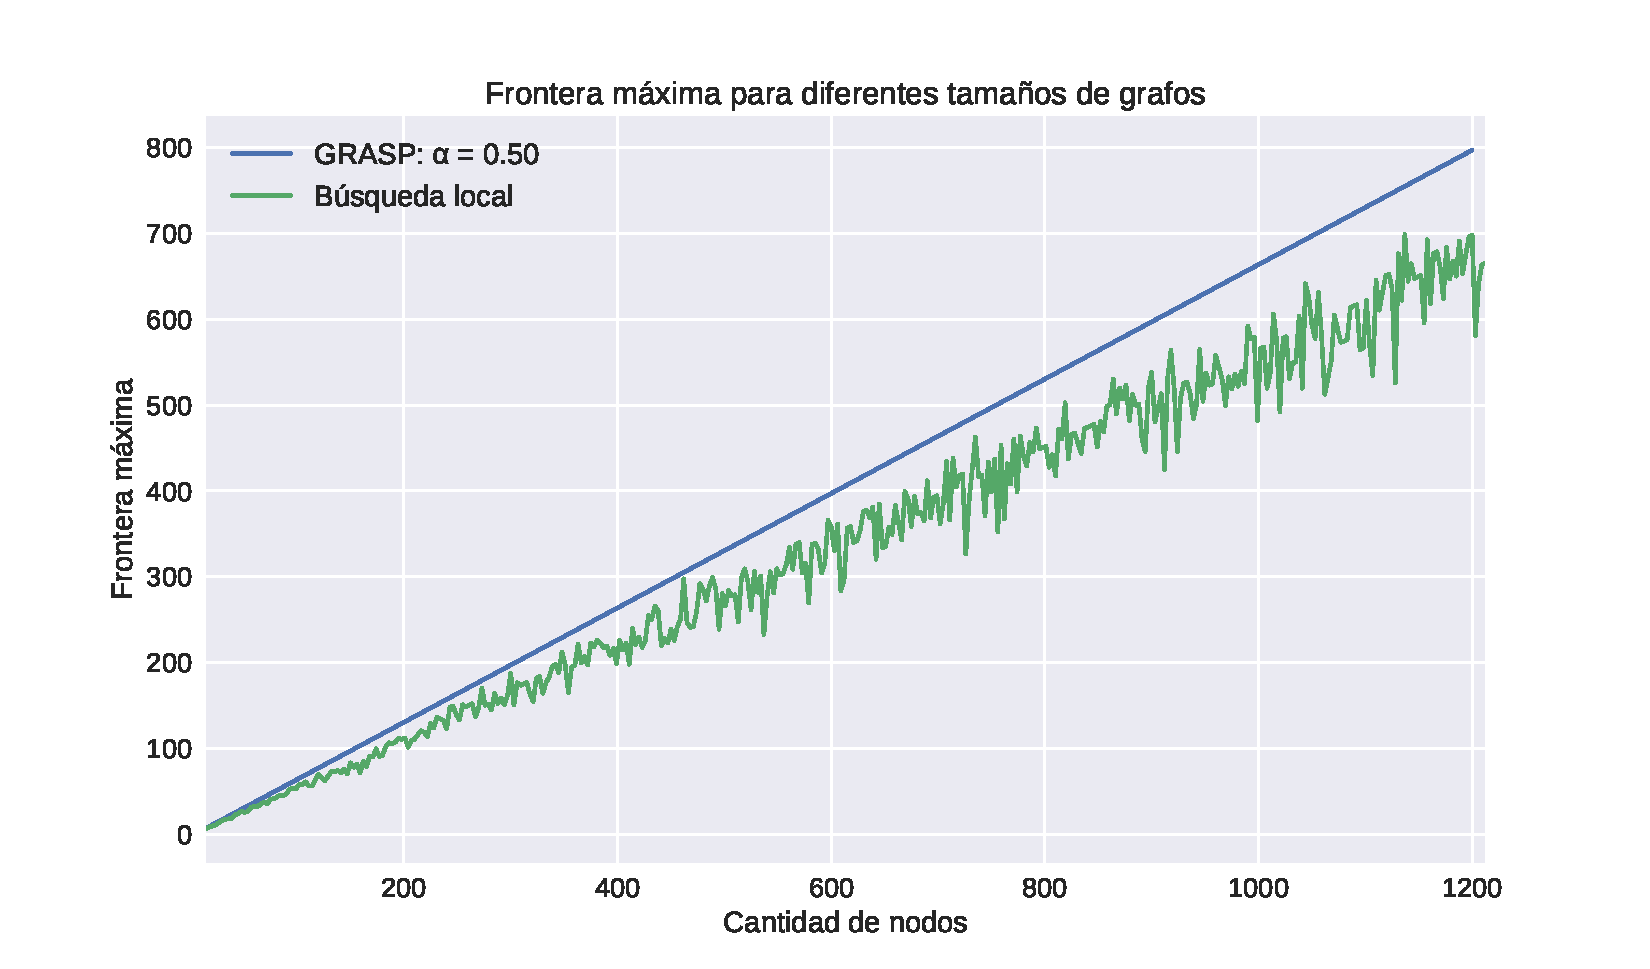
\includegraphics[width=1\textwidth]{informe/imgs/exp_malo_frontera_grasp_local.pdf}
}

{\centering
    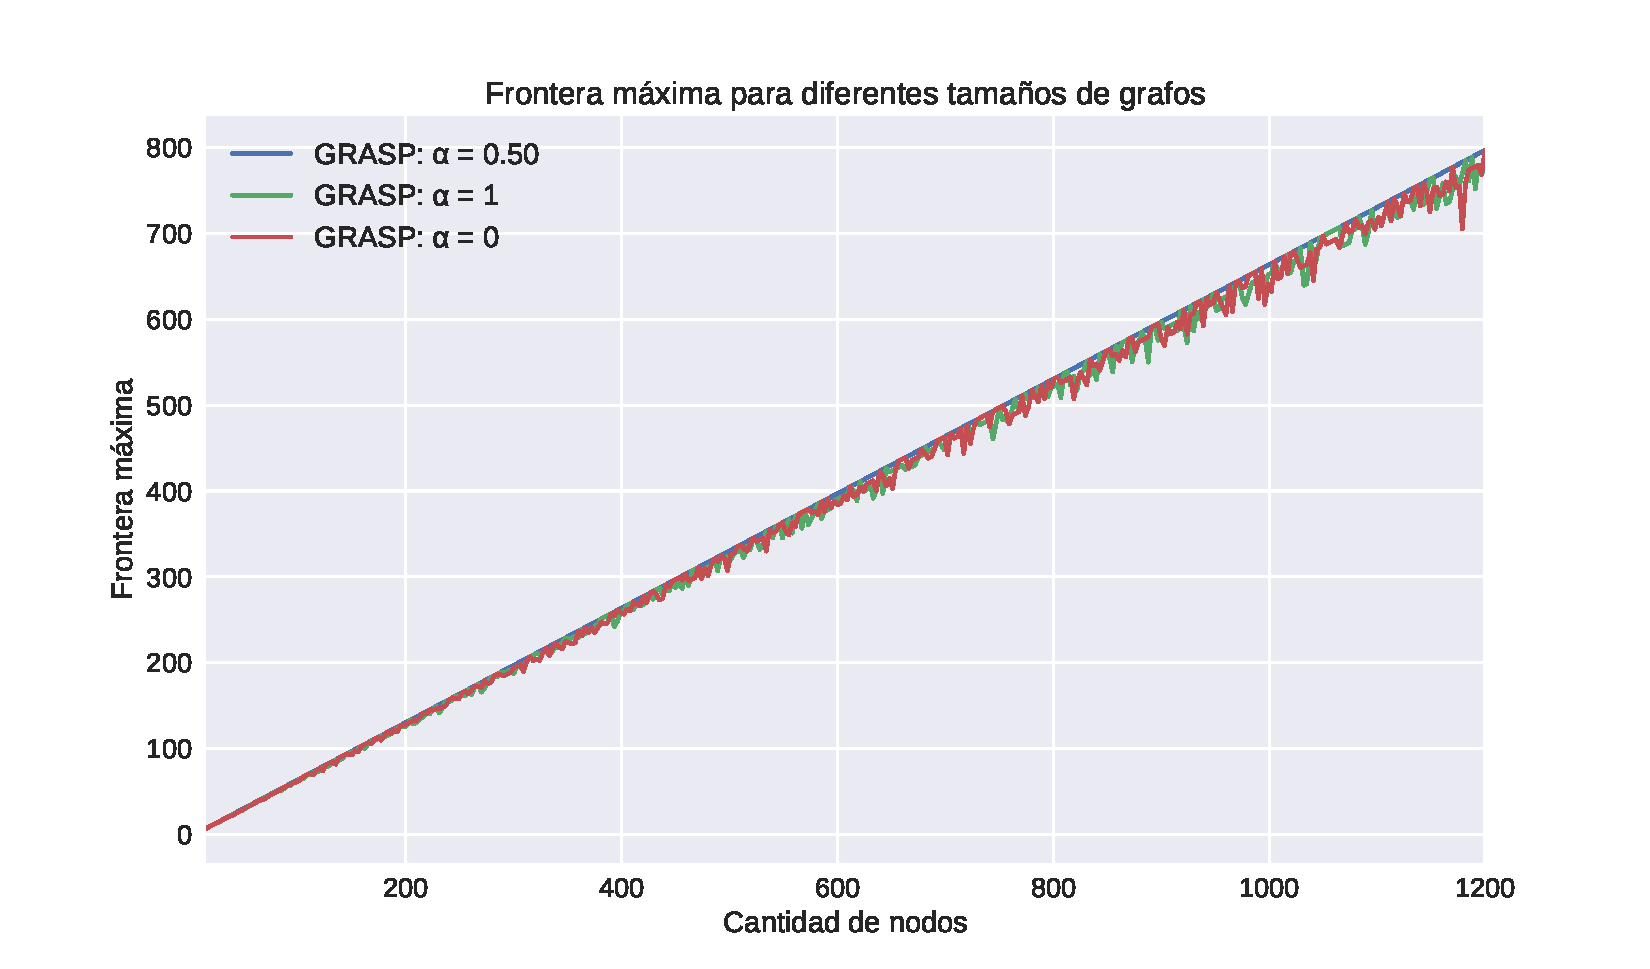
\includegraphics[width=1\textwidth]{informe/imgs/exp_malo_frontera_grasp.pdf}
}

{\centering
    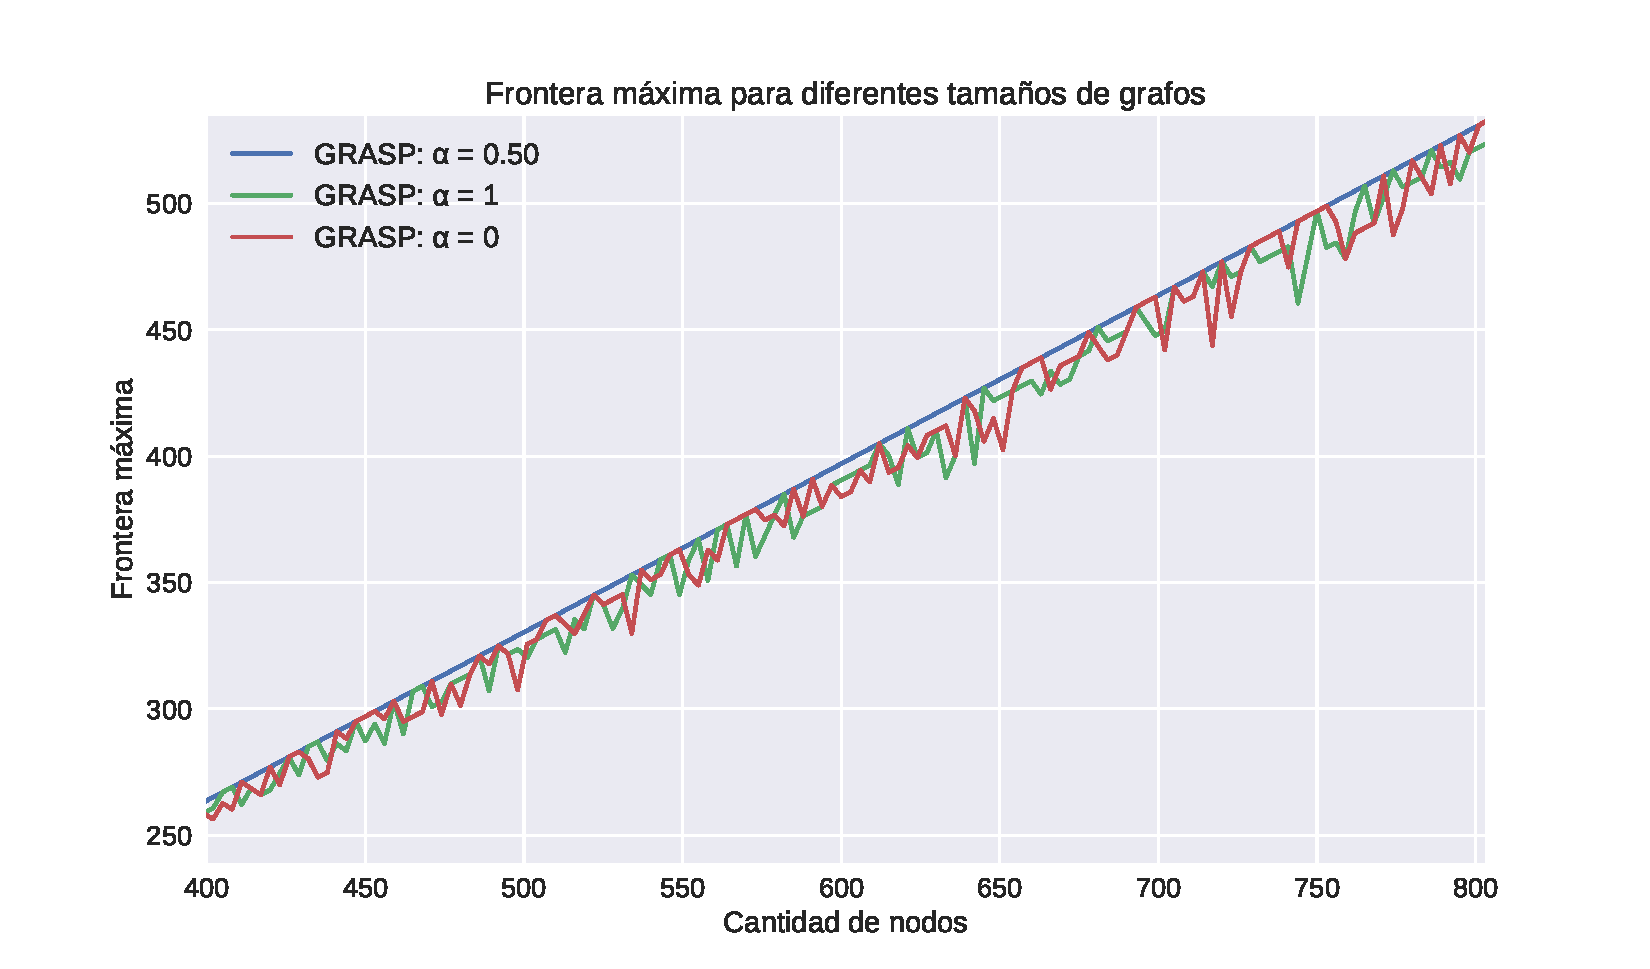
\includegraphics[width=1\textwidth]{informe/imgs/exp_malo_frontera_grasp_zoom.pdf}
    \captionof{figure}{$\uparrow$ Zoom del gráfico anterior}
}

{\centering
    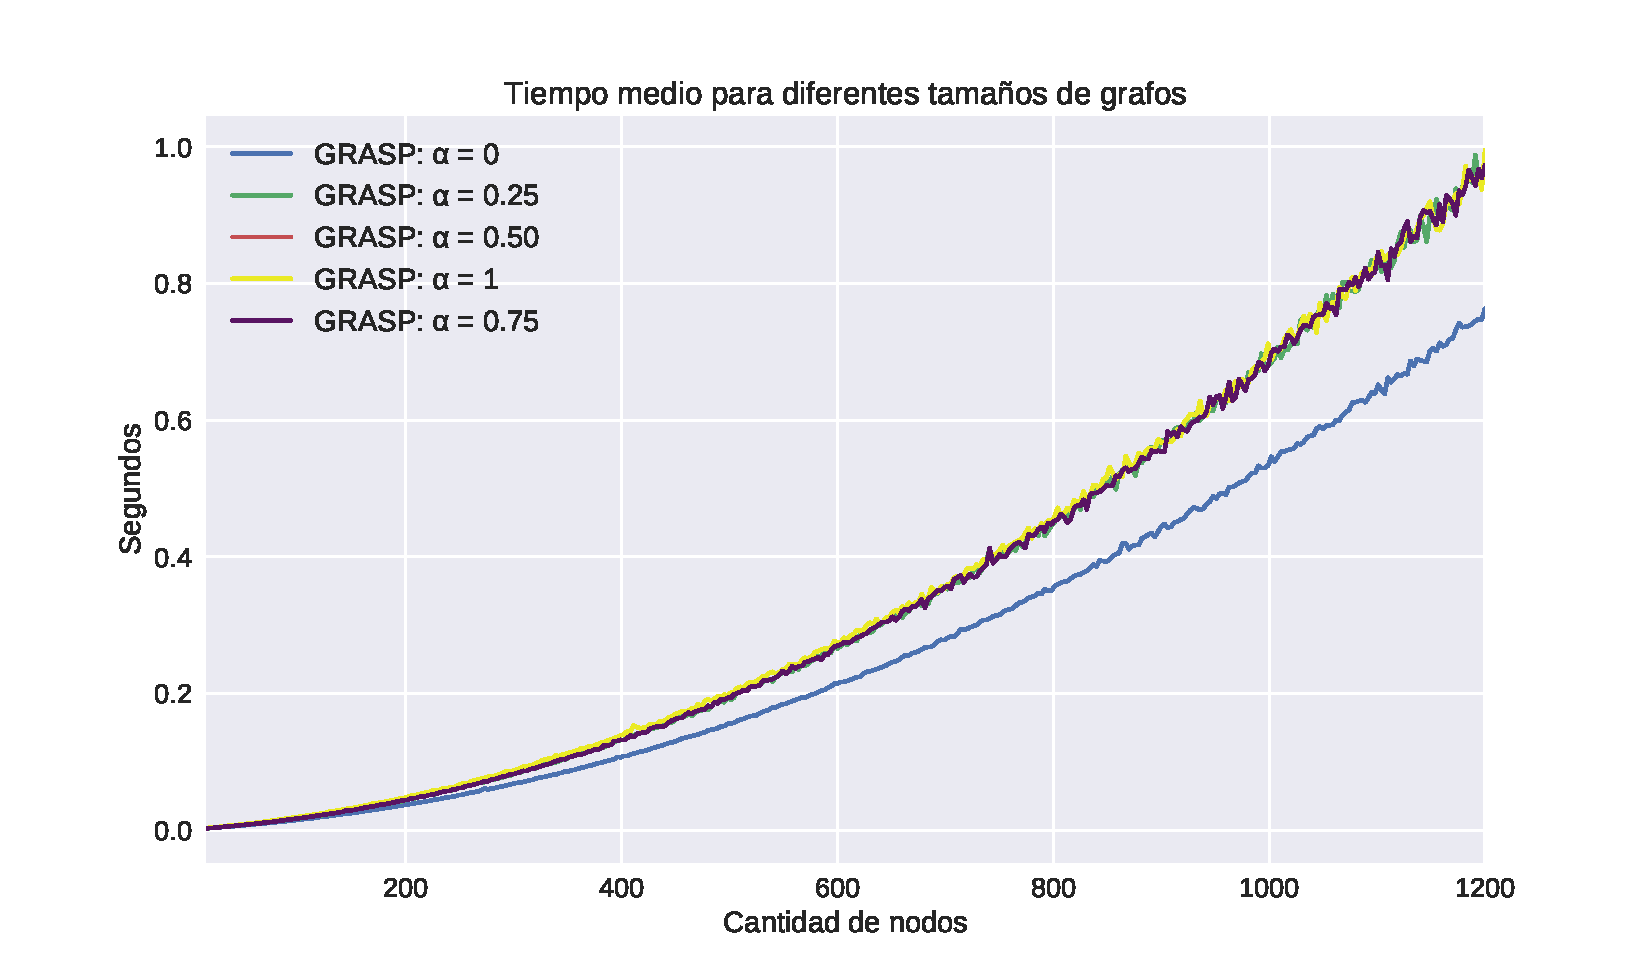
\includegraphics[width=1\textwidth]{informe/imgs/exp_malo_tiempo_grasp.pdf}
}